% http://en.wikibooks.org/wiki/LaTeX/Title_Creation
% Adjusted for EPFL template


\begin{titlepage}

\begin{center}

\raisebox{2cm}[-2cm][-2cm]{
\hspace{-1.5cm}

  \footnotesize
  \begin{tabular}{@{\hspace{10pt}}l@{\hspace{0pt}} l@{\hspace{10pt}}}
  %  \cline{0-0}     &\multirow{5}{*}{\hspace{10pt}\raisebox{-1ex}{
\includegraphics[width=0.4\columnwidth]{CERN-logo}}}\\
    \multirow{5}{*}{\hspace{10pt}\raisebox{-1ex}{
\includegraphics[height=0.2\textheight]{CERN-logo}}}    & \multirow{5}{*}{\hspace{10pt}\raisebox{-1ex}{
\includegraphics[width=0.4\columnwidth]{EPFL_LOG_QUADRI_Red}}}\\

         \\
    \\
    \raisebox{1.2ex}{INSTITUT DE MICROTECHNIQUE | Laboratoire de Microsyst�mes} \\
    %\scriptsize CH -- 1015 LAUSANNE \\

  \end{tabular}%
}

\vspace{1\baselineskip}
\Huge

\newcommand{\HRule}{\rule{\linewidth}{0.3mm}}


    {\huge \bfseries  A monolithic microrobotic arm \\ in silicon} \\
    {\Large \bfseries  Microrobot monolithique en silicium} \\
	\vspace{3mm}    
    \textsc{\Large Projet de Semestre} \Large (Automne 2009) \\
    \Large Section Microtechnique
    
    %\HRule \\[0.2cm]
	
	\vspace{3mm}
	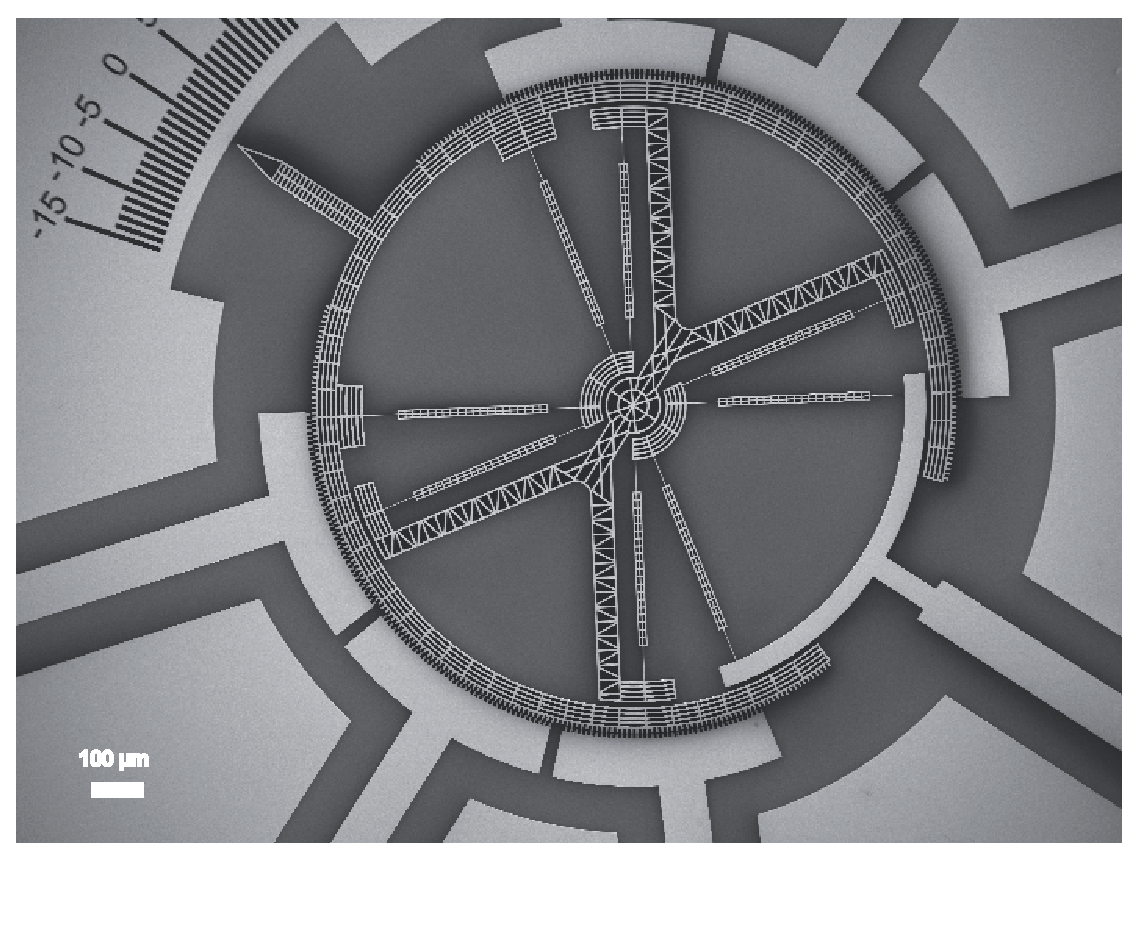
\includegraphics[height=6 cm]{fig_couverture}
	\vspace{3mm}
	\HRule 
	
	\emph{Auteur:} \\
	Marc \textsc{Stranczl}\\
    \vspace{0.5cm}
    \emph{Sous la supervision de:} \\   

    Prof. Martinus \textsc{Gijs}, LMIS2 \\   
    Dr. Christophe \textsc{Yamahata}, LMIS 2\\

	\vspace{0.5cm}
    % Bottom of the page
    \emph{Remis le: 8 janvier 2010}
	%{\large \today}


\end{center}


\end{titlepage}

\newpage
\thispagestyle{empty}
\mbox{}